\documentclass[final]{beamer}\usepackage[]{graphicx}\usepackage[]{color}
%% maxwidth is the original width if it is less than linewidth
%% otherwise use linewidth (to make sure the graphics do not exceed the margin)
\makeatletter
\def\maxwidth{ %
  \ifdim\Gin@nat@width>\linewidth
    \linewidth
  \else
    \Gin@nat@width
  \fi
}
\makeatother

\definecolor{fgcolor}{rgb}{0.345, 0.345, 0.345}
\newcommand{\hlnum}[1]{\textcolor[rgb]{0.686,0.059,0.569}{#1}}%
\newcommand{\hlstr}[1]{\textcolor[rgb]{0.192,0.494,0.8}{#1}}%
\newcommand{\hlcom}[1]{\textcolor[rgb]{0.678,0.584,0.686}{\textit{#1}}}%
\newcommand{\hlopt}[1]{\textcolor[rgb]{0,0,0}{#1}}%
\newcommand{\hlstd}[1]{\textcolor[rgb]{0.345,0.345,0.345}{#1}}%
\newcommand{\hlkwa}[1]{\textcolor[rgb]{0.161,0.373,0.58}{\textbf{#1}}}%
\newcommand{\hlkwb}[1]{\textcolor[rgb]{0.69,0.353,0.396}{#1}}%
\newcommand{\hlkwc}[1]{\textcolor[rgb]{0.333,0.667,0.333}{#1}}%
\newcommand{\hlkwd}[1]{\textcolor[rgb]{0.737,0.353,0.396}{\textbf{#1}}}%

\usepackage{framed}
\makeatletter
\newenvironment{kframe}{%
 \def\at@end@of@kframe{}%
 \ifinner\ifhmode%
  \def\at@end@of@kframe{\end{minipage}}%
  \begin{minipage}{\columnwidth}%
 \fi\fi%
 \def\FrameCommand##1{\hskip\@totalleftmargin \hskip-\fboxsep
 \colorbox{shadecolor}{##1}\hskip-\fboxsep
     % There is no \\@totalrightmargin, so:
     \hskip-\linewidth \hskip-\@totalleftmargin \hskip\columnwidth}%
 \MakeFramed {\advance\hsize-\width
   \@totalleftmargin\z@ \linewidth\hsize
   \@setminipage}}%
 {\par\unskip\endMakeFramed%
 \at@end@of@kframe}
\makeatother

\definecolor{shadecolor}{rgb}{.97, .97, .97}
\definecolor{messagecolor}{rgb}{0, 0, 0}
\definecolor{warningcolor}{rgb}{1, 0, 1}
\definecolor{errorcolor}{rgb}{1, 0, 0}
\newenvironment{knitrout}{}{} % an empty environment to be redefined in TeX

\usepackage{alltt}
\usepackage[orientation = landscape, size = a0, scale = 1.4]{beamerposter}

\usepackage{amsmath, amsthm}
\usepackage[]{graphicx}
\usepackage{parskip, microtype}
\usepackage{caption, subcaption, multirow}
\usepackage{morefloats, hyperref}
\usepackage{rotating, longtable}
\usepackage[sort&compress, numbers]{natbib}

\usetheme{confposter}


\newlength{\sepwid}
\newlength{\onecolwid}
\newlength{\twocolwid}
\newlength{\threecolwid}
\setlength{\paperwidth}{48in} % A0 width: 46.8in
\setlength{\paperheight}{36in} % A0 height: 33.1in
\setlength{\sepwid}{0.024\paperwidth} % Separation width (white space) between columns
\setlength{\onecolwid}{0.22\paperwidth} % Width of one column
\setlength{\twocolwid}{0.464\paperwidth} % Width of two columns
\setlength{\threecolwid}{0.708\paperwidth} % Width of three columns

\def\newblock{\hskip .11em plus .33em minus .07em}





\title{Cosmopolitan and endemism dynamics of terrestrial Cenozoic mammals} 
\author{Peter D Smits}
\institute{Committee on Evolutionary Biology, University of Chicago}
\IfFileExists{upquote.sty}{\usepackage{upquote}}{}

\begin{document}
\begin{frame}[t]
  \begin{columns}[t]
    \begin{column}{\onecolwid}
    \begin{block}{Extended abstract}
% trophic structure change through time
%   constituent taxa
%   paleo record
%     sampling (lack of abundance in terrestrial systems)
%     site occupancy/distribution
%   evolution of community
%     Damuth1982 on preservation of structure
%     Roopnarine2010,Roopnarine2012b,Roopnarine2007,
%     Roopnarine2006,Mitchell2012,Angielczyk2005
%
% distribution of organisms across the landscape
% how does life history affect distribution?
% how does taxonomic distribution change over time
%   life history characters
%     diet
%     life habit/locomotor category
%   abiotic factors
%     climate Zachos2001,Zachos2008

        Community structure plays a fundamental roll in determining ecological dynamics. 
        Evolutionary paleoecology is defined as the study of the consequences of ecological properties, roles and strategies at any and all levels on the evolutionary process \citep{Kitchell1985a}. Biotic and abiotic interactions change over time and understanding their interplay, both biotic--biotic and biotic--abiotic, is important for determining which ecological properties affect macroevolutionary trends and how.
        How the taxonomic composition of communities have changed over time is of interest because community composition determines the range of plausible biotic interactions. Additionally, if change in taxonomic and life history composition is correlated with abiotic factors such as temperature then our knowledge of the pattern of mammalian evolution in the past and in the future might be better constrained.

        Previous work on mammalian site similarity has focused on distributions of terrestrial mammals in the Neogene Old World \citep{Jernvall2002,Jernvall2004}. 
        Here, I expand that analysis to the entire Cenozoic of North America and both dietary and locomotor categories of terrestrial mammals. Additionally, I analyze if shifts in taxonomic and life history composition are correlated with climatic change.
        To measure taxonomic distribution as a proxy for community structure, biogeographic networks were constructed between species and formation occurrence. Four different measures of biogeographic network structure were used to assess changes in mammalian community structure through the Cenozoic.
      \end{block}

      \begin{footnotesize}
      \begin{block}{Methods}
        Mammalian taxonomic occurrence information was obtained from the Paleobiology Database (\url{http://www.paleodb.org}). Taxonomic occurrence information was restricted to only mammals occurring in North America during the Cenozoic. Ambiguously identified taxa were excluded from all analyses (e.g. aff., cf., ?). Temporal, geologic, and life history information was also compiled. Because terrestrial assemblages across the Cenozoic do not preserve as complete a record of community structure, abundance distributions were not analyzed.

        %biogeographic networks
        Following \citet{Sidor2013} and \citet{Vilhena2013}, bipartite taxa-locality networks were constructed. Here, taxa were defined as the occurrence list of all unique species and locality was defined as formation. Biogeographic networks were constructed for uniform 2 My bins from the K/Pg to the Recent which were chosen for multiple reasons. Prior analysis has shown that the mammalian fossil record of the Cenozoic of North America is resolvable to approximately 1 My \citep{Alroy1996a,Alroy2000g}. Here, because I am interested in diversity dynamics across multiple formations, I used a bin width of 2 My to allow for every bin to be represented by minimum of two formations.

        Biogeographic network structure was assessed using four previously defined measures \citep{Sidor2013}: average number of locality occurrences per taxon, biogeographic connectedness, code length, and average number of endemic taxa per locality. 

        Climate change, specifically temperature, was estimated using a benthic foram \(\delta O^{18}\) isotope curve of the whole Cenozoic \citep{Zachos2008}. Bin \(\delta O^{18}\) values were calculated as the average of all data points occuring in that bin.

        Correlation tests were done between between the first differences of all biogeographic summary statistic time series and the \(\delta O^{18}\) curve. 

      \end{block}
      \end{footnotesize}

    \end{column}

    \begin{column}{\twocolwid}
      \begin{columns}[t,totalwidth = \twocolwid]
        \begin{column}{\onecolwid}
          \begin{block}{\(\delta O^{18}\)}
            \begin{figure}[ht]
              \centering
              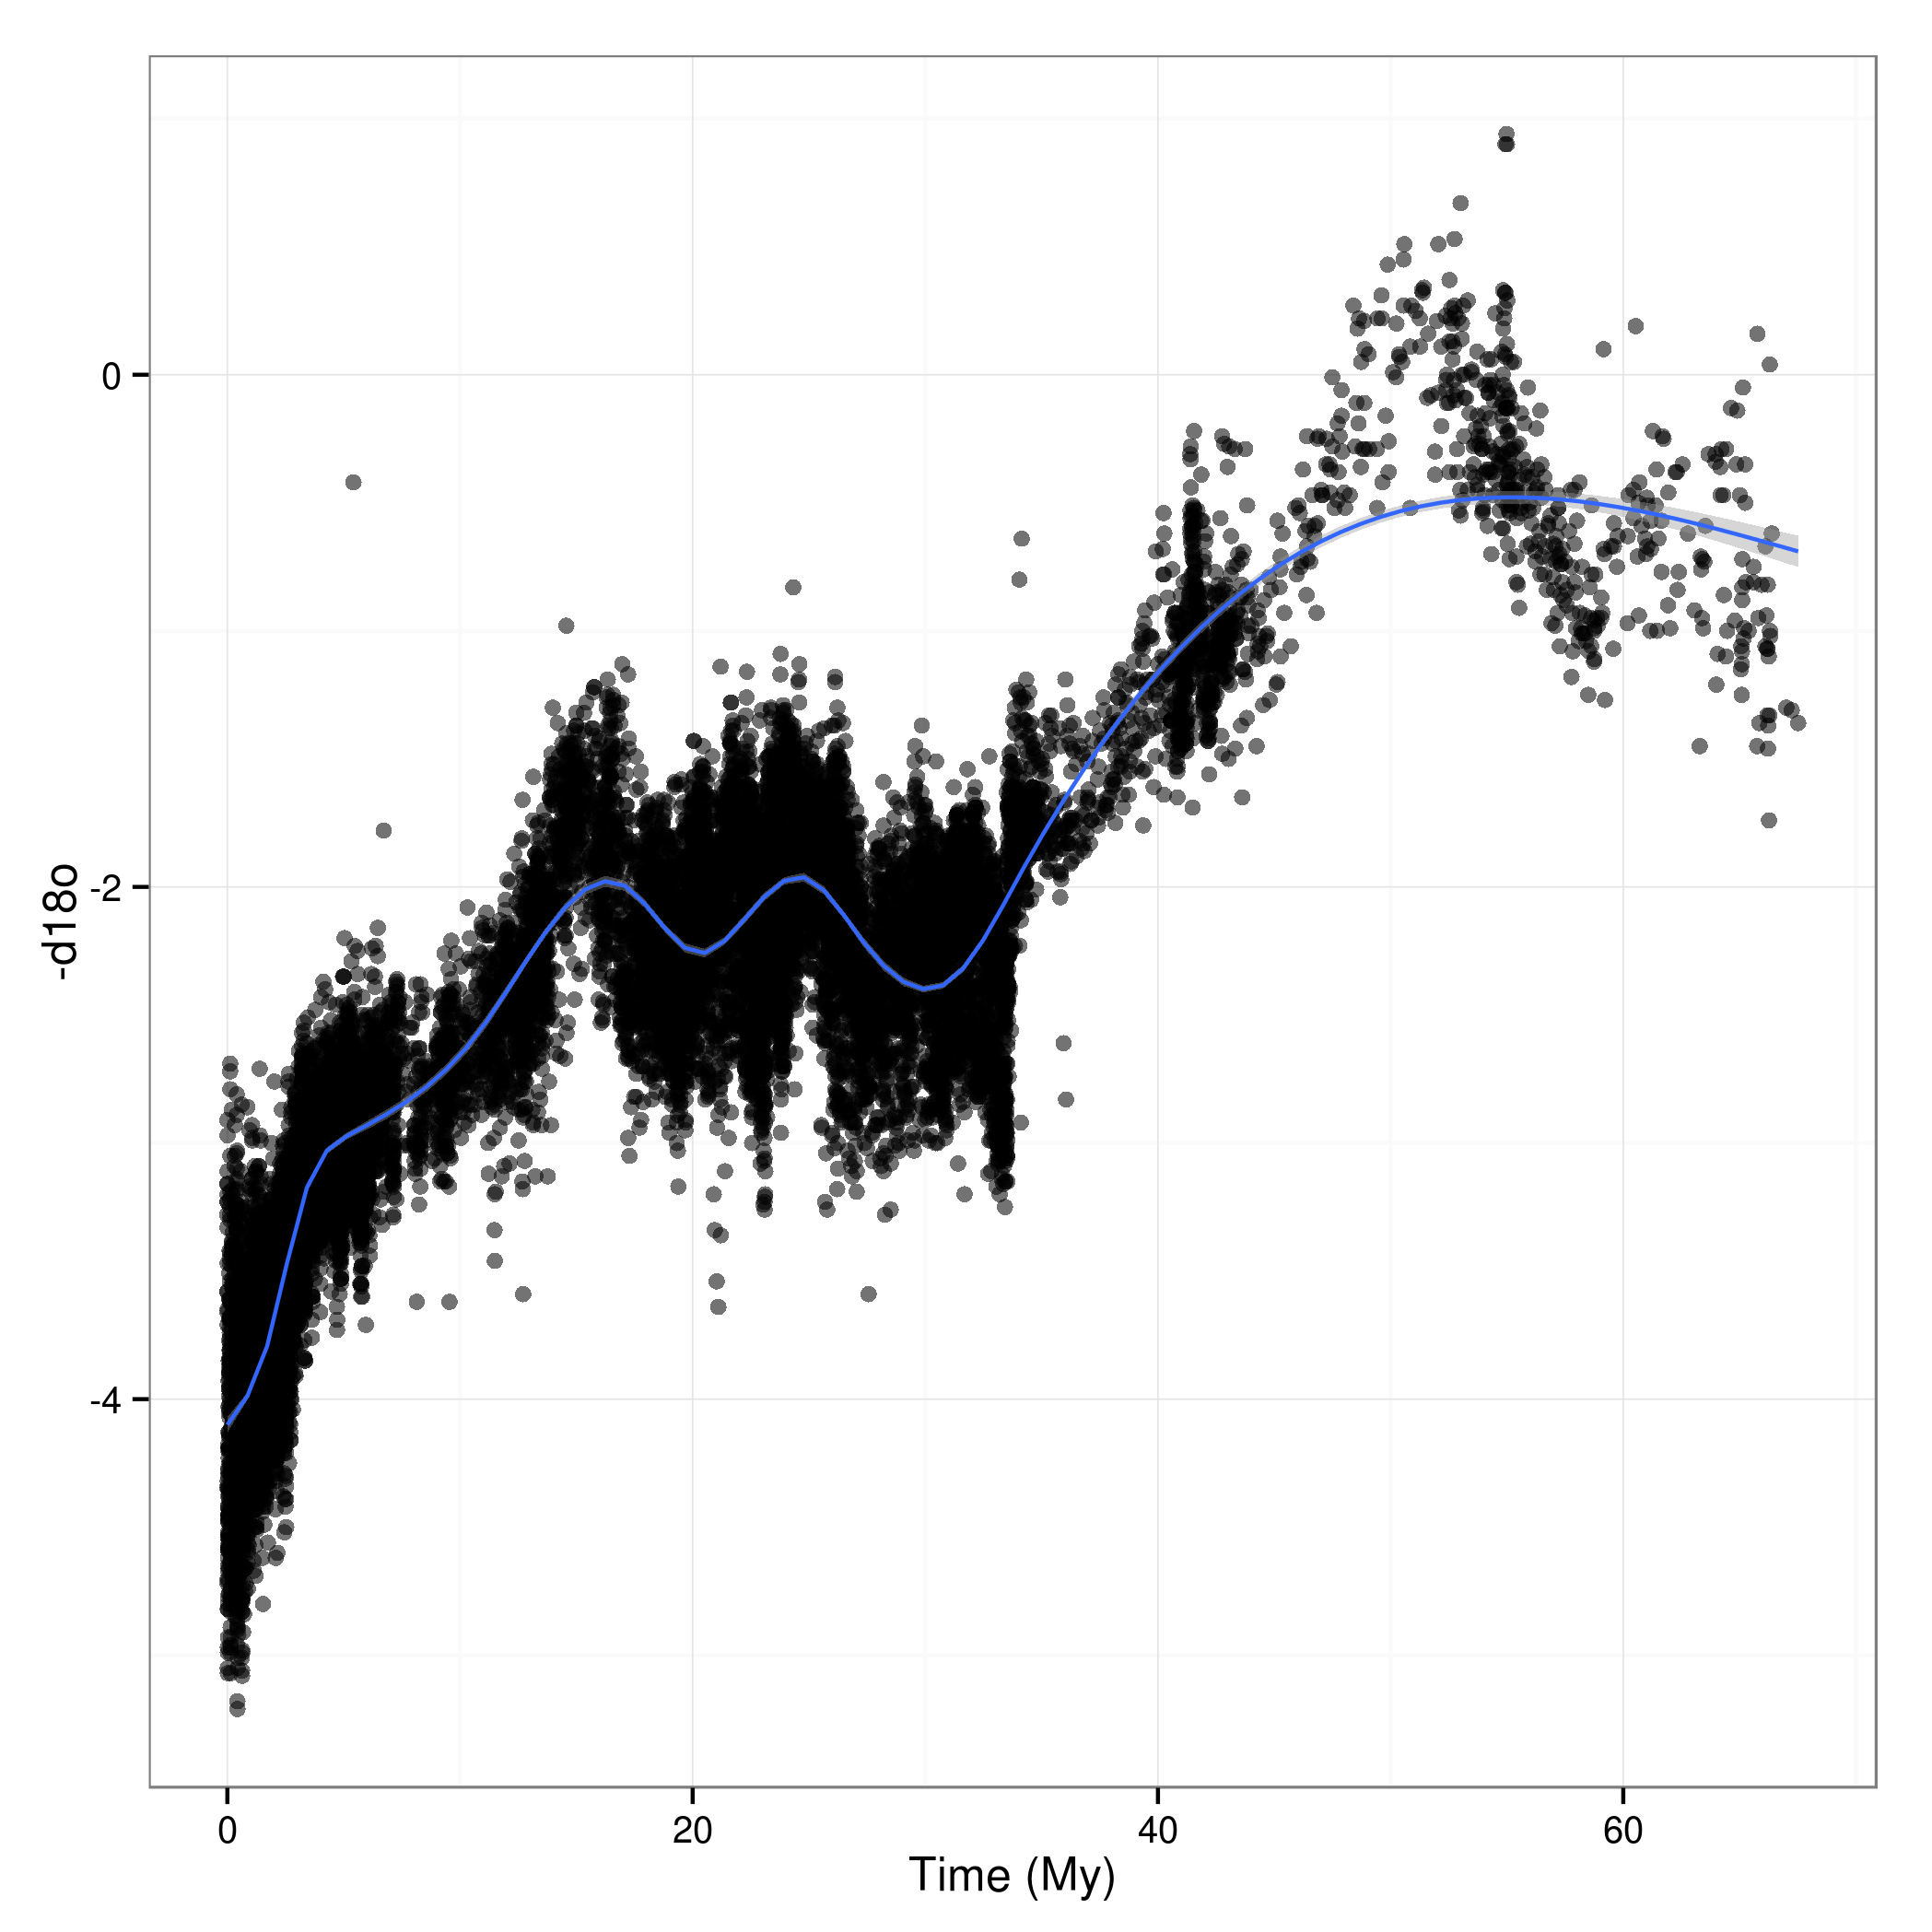
\includegraphics[height = 0.2\textheight]{figure/zachos}
              \caption{Oxygen curve \citep{Zachos2008} with fitted GAM to illustrate overall structure.}
              \label{fig:zac}
            \end{figure}
          \end{block}
        \end{column}

        \begin{column}{\onecolwid}
          \begin{block}{Biogeographic structure}
            \begin{figure}[ht]
              \begin{center}
                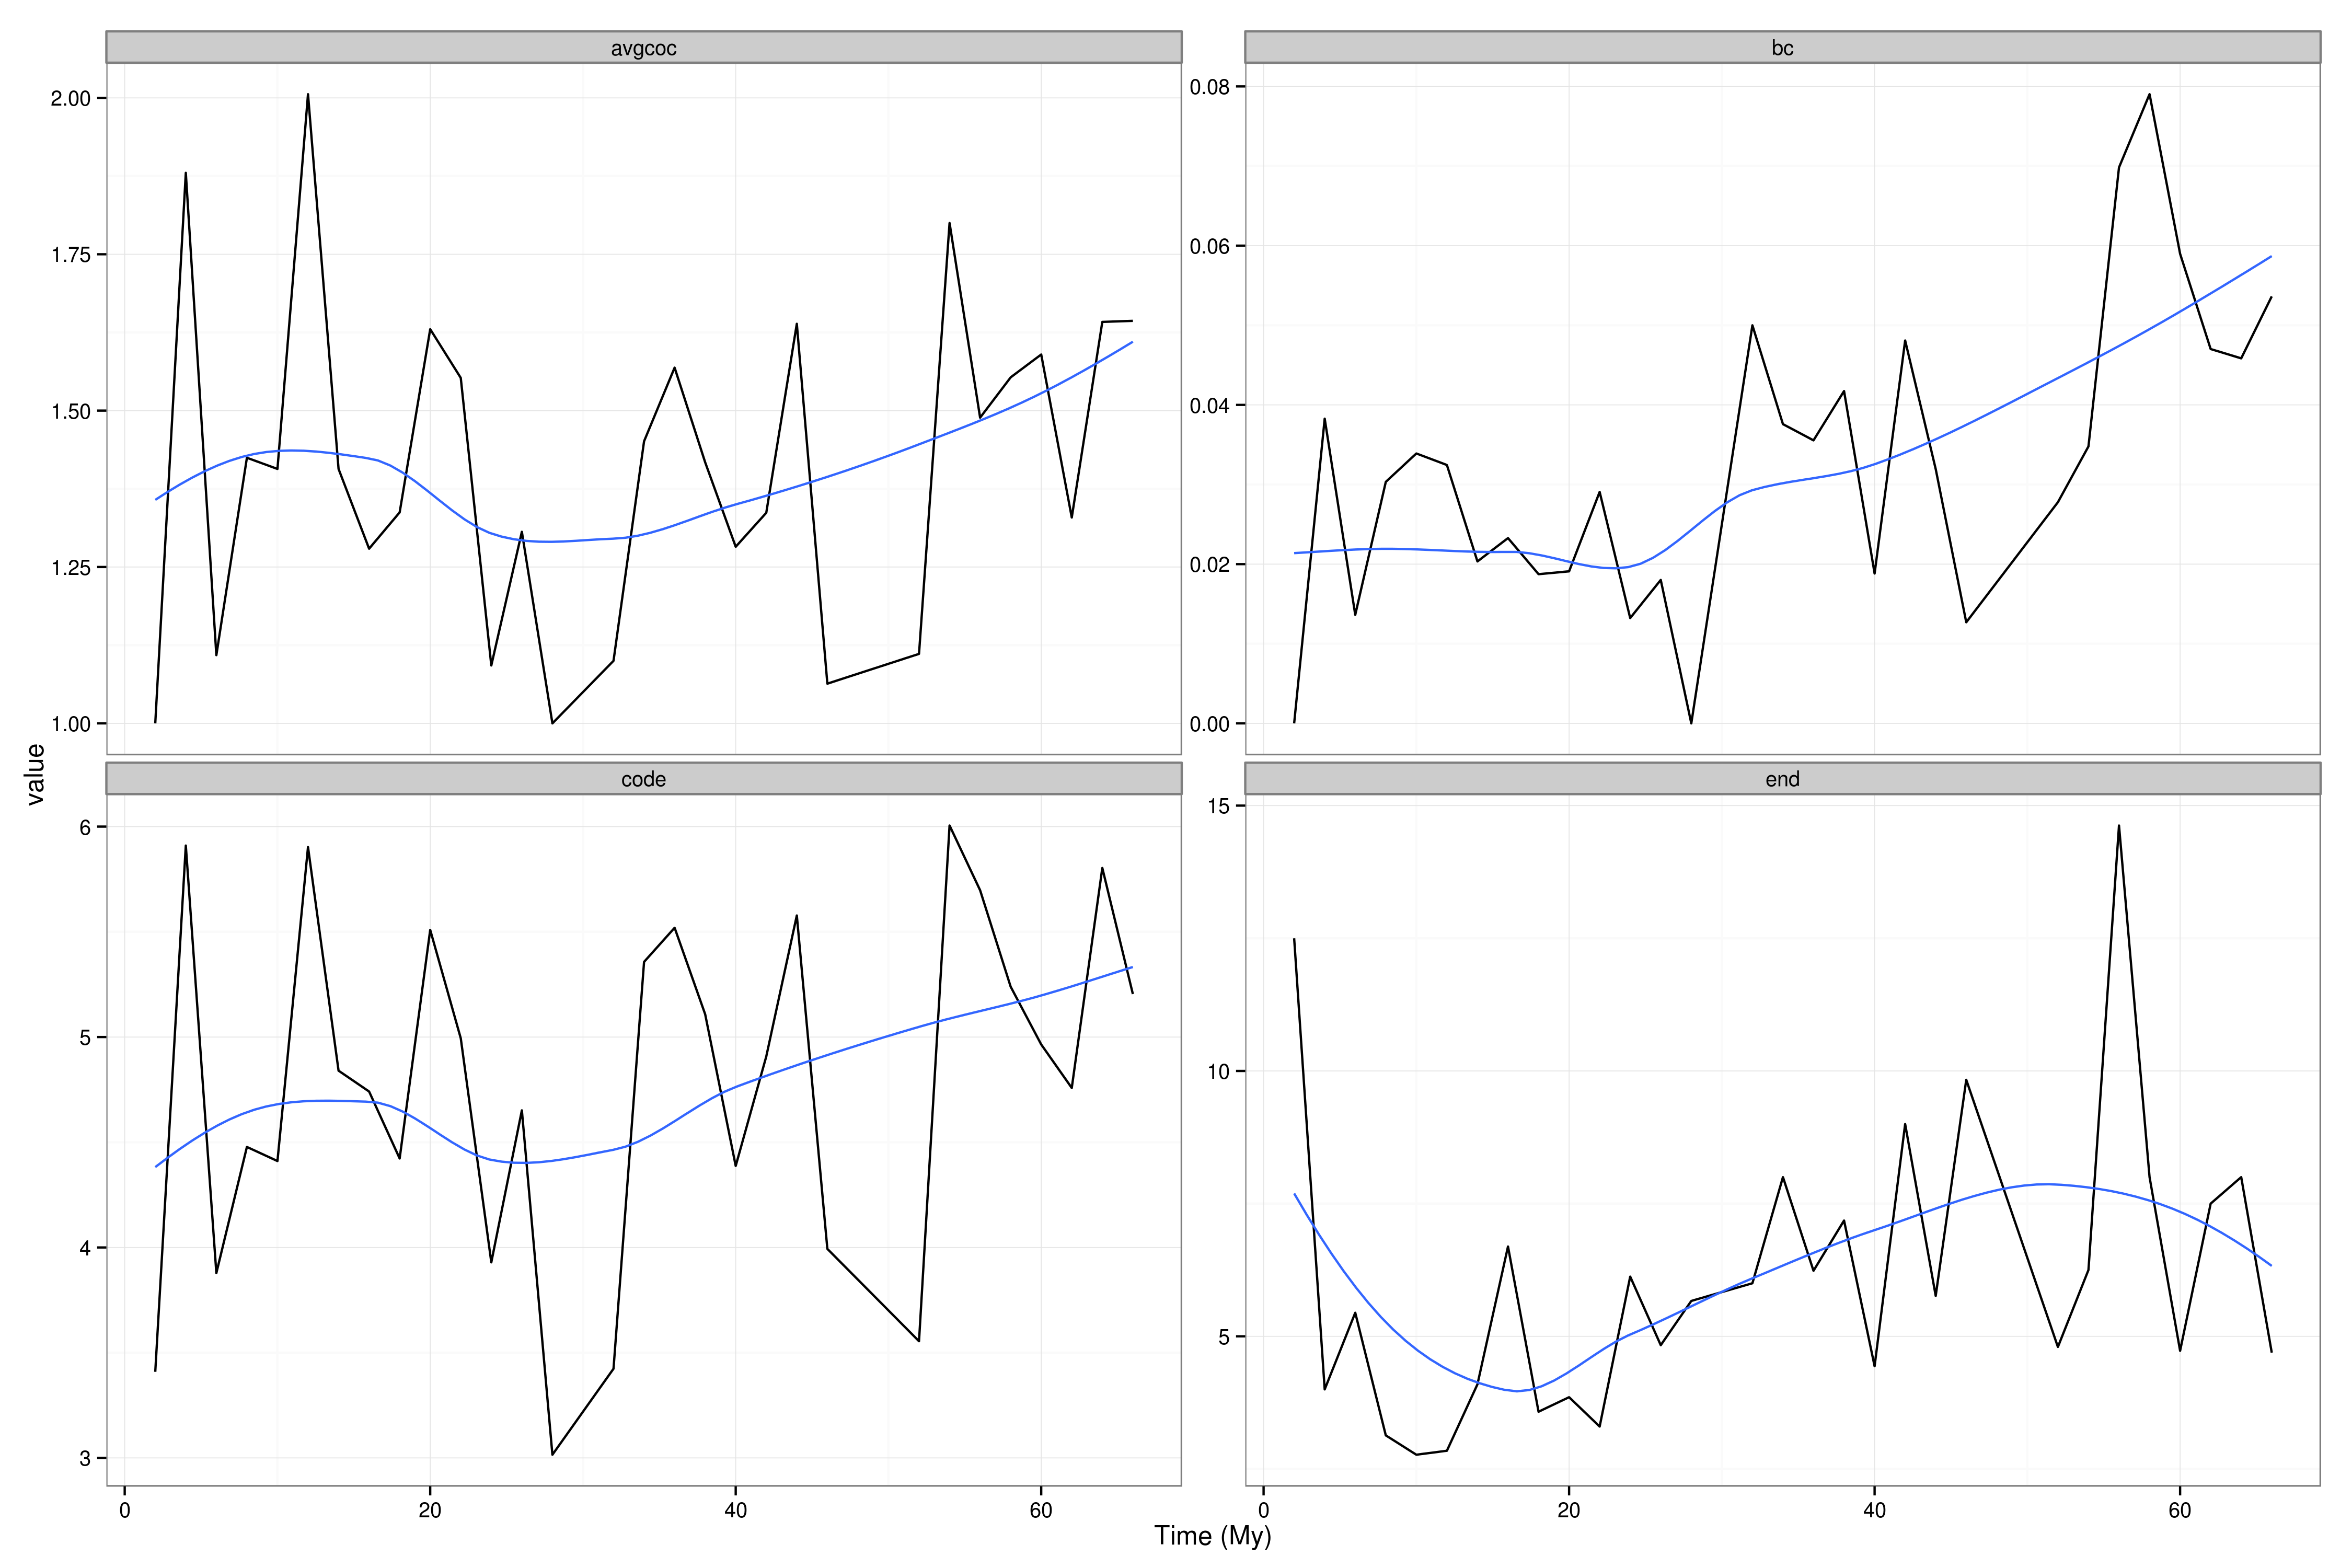
\includegraphics[height = 0.2\textheight]{figure/gen_bin}
              \end{center}
              \caption{Summary statistics of the mammal wide biogeographic networks for every 2 My bin.}
              \label{fig:net_gen}
            \end{figure}
          \end{block}
        \end{column}
      \end{columns}

      \begin{alertblock}{Life history dynamics}
        \begin{figure}[ht]
          \begin{center}
            \begin{subfigure}[b]{\onecolwid}
              \centering
              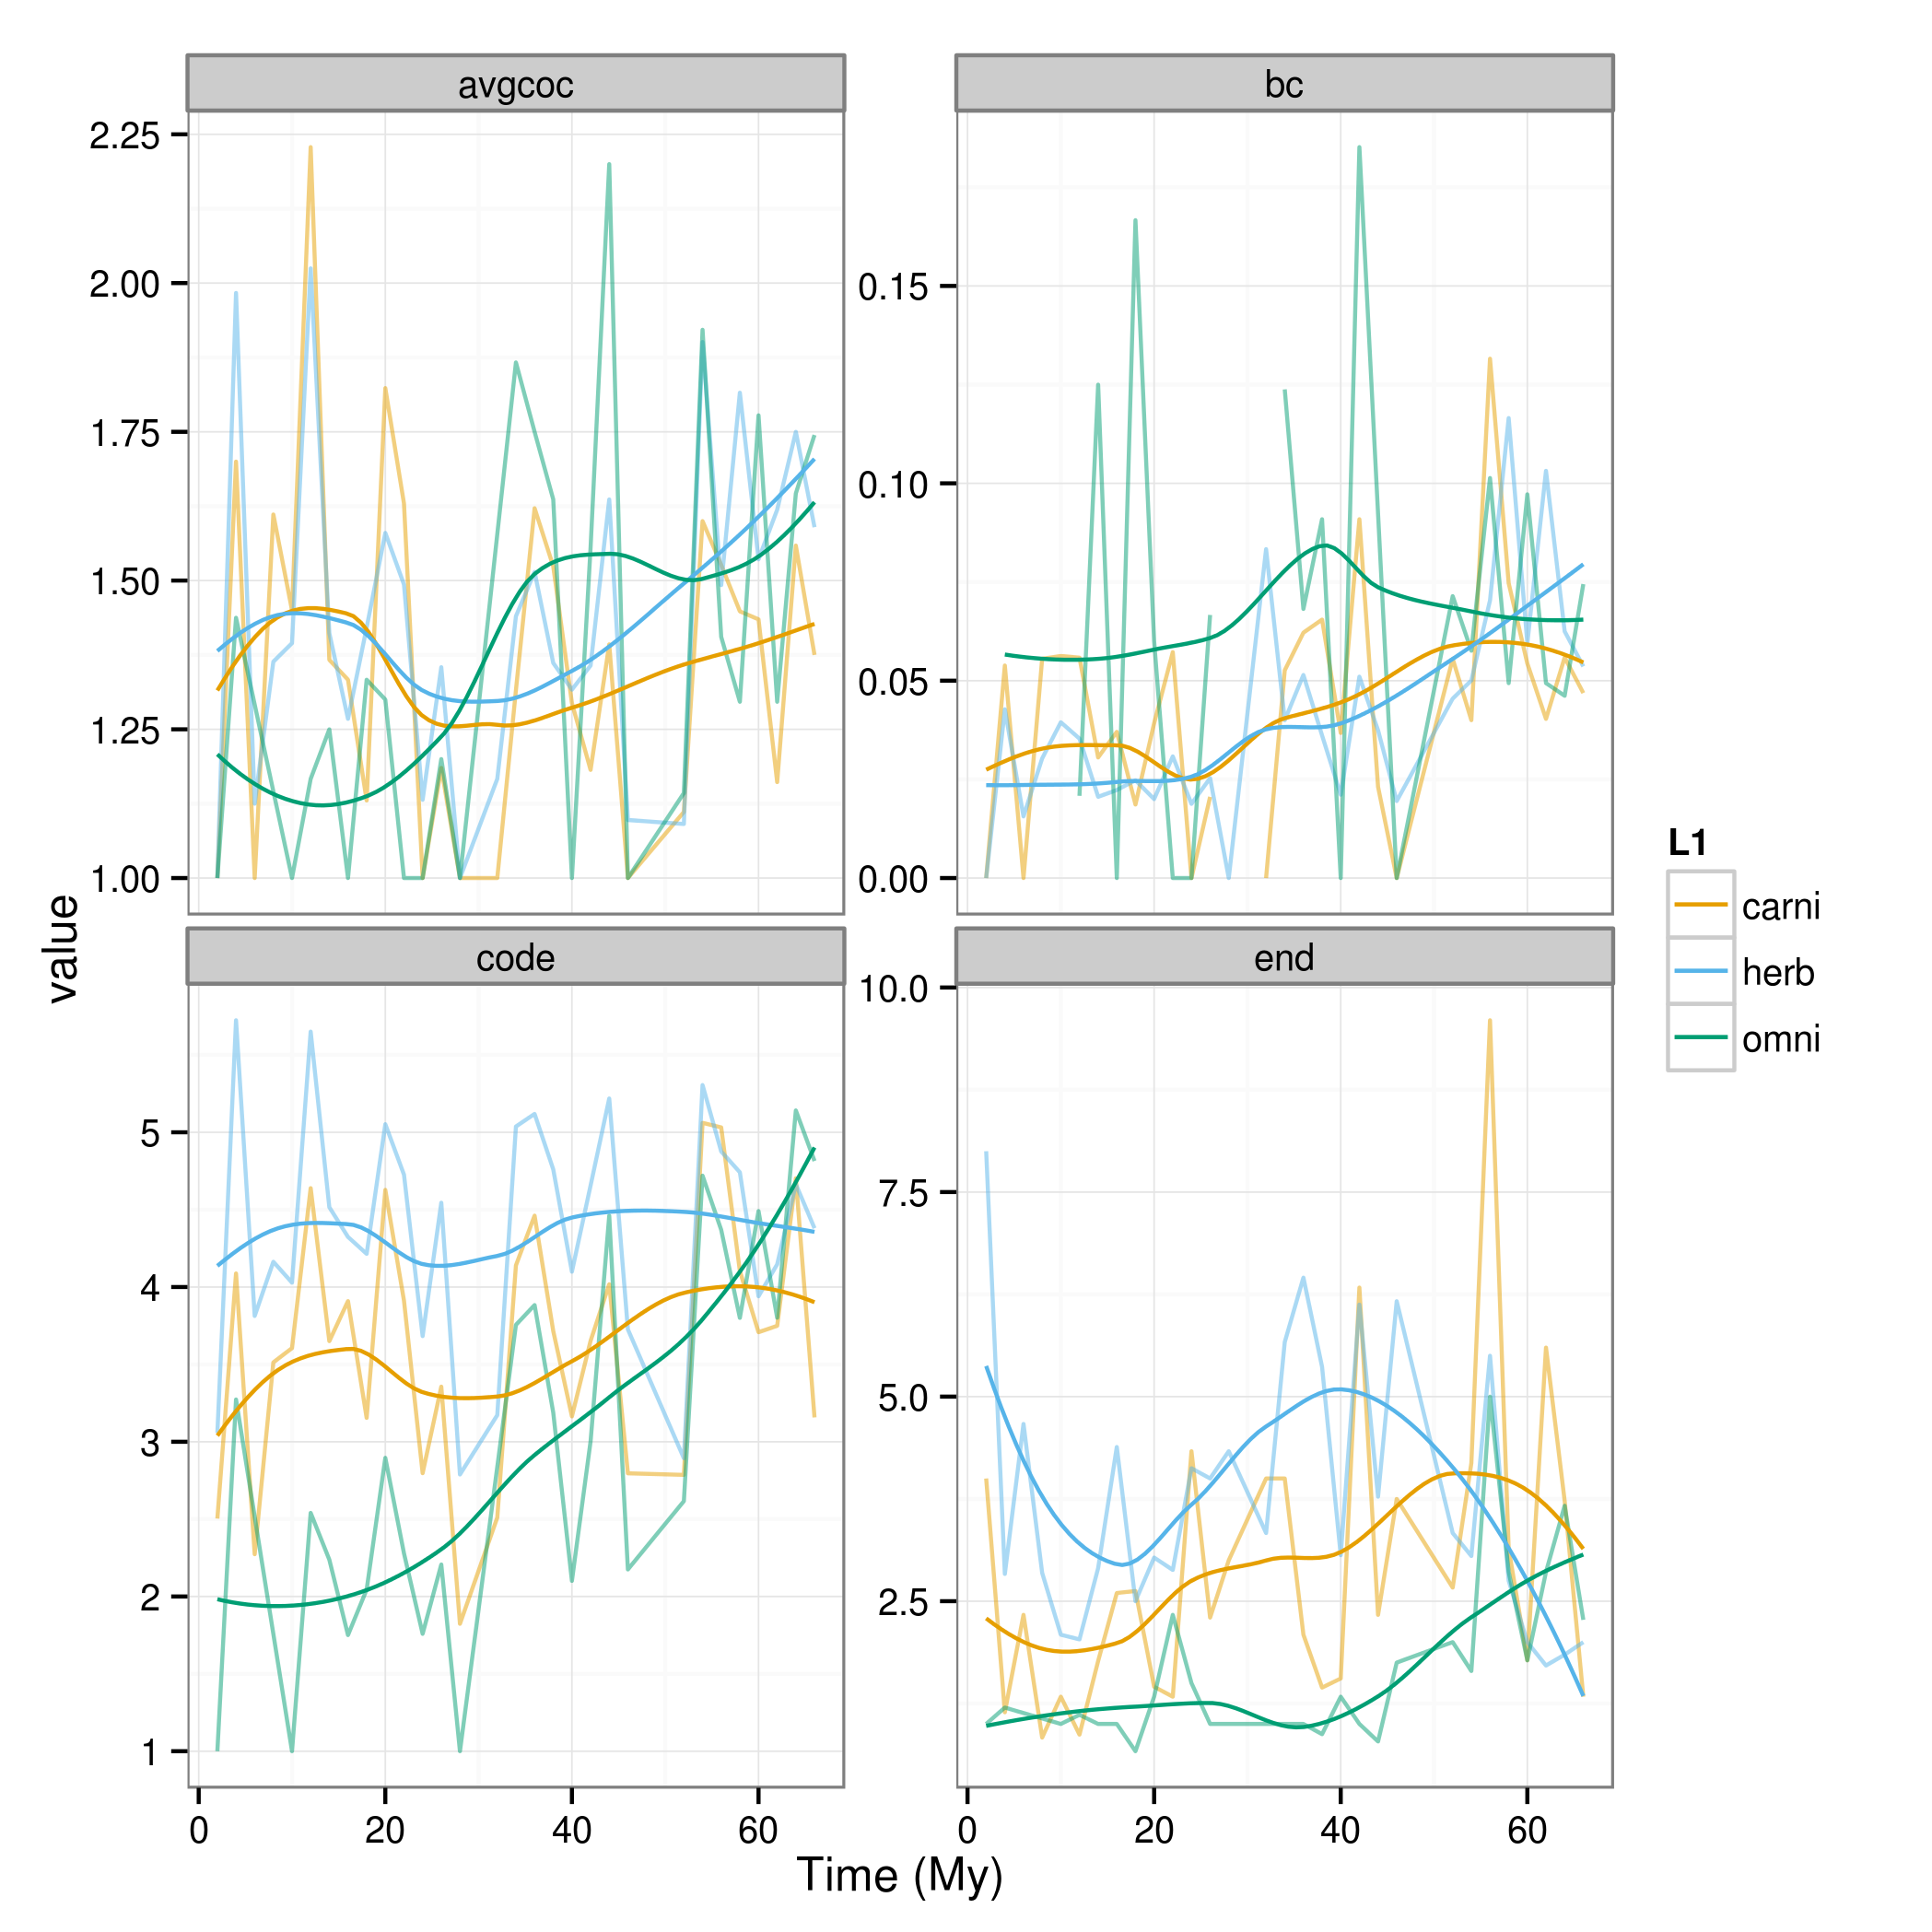
\includegraphics[width = 0.8\onecolwid]{figure/diet_bin}
              \label{fig:net_diet}
            \end{subfigure}
            \begin{subfigure}[b]{\onecolwid}
              \centering
              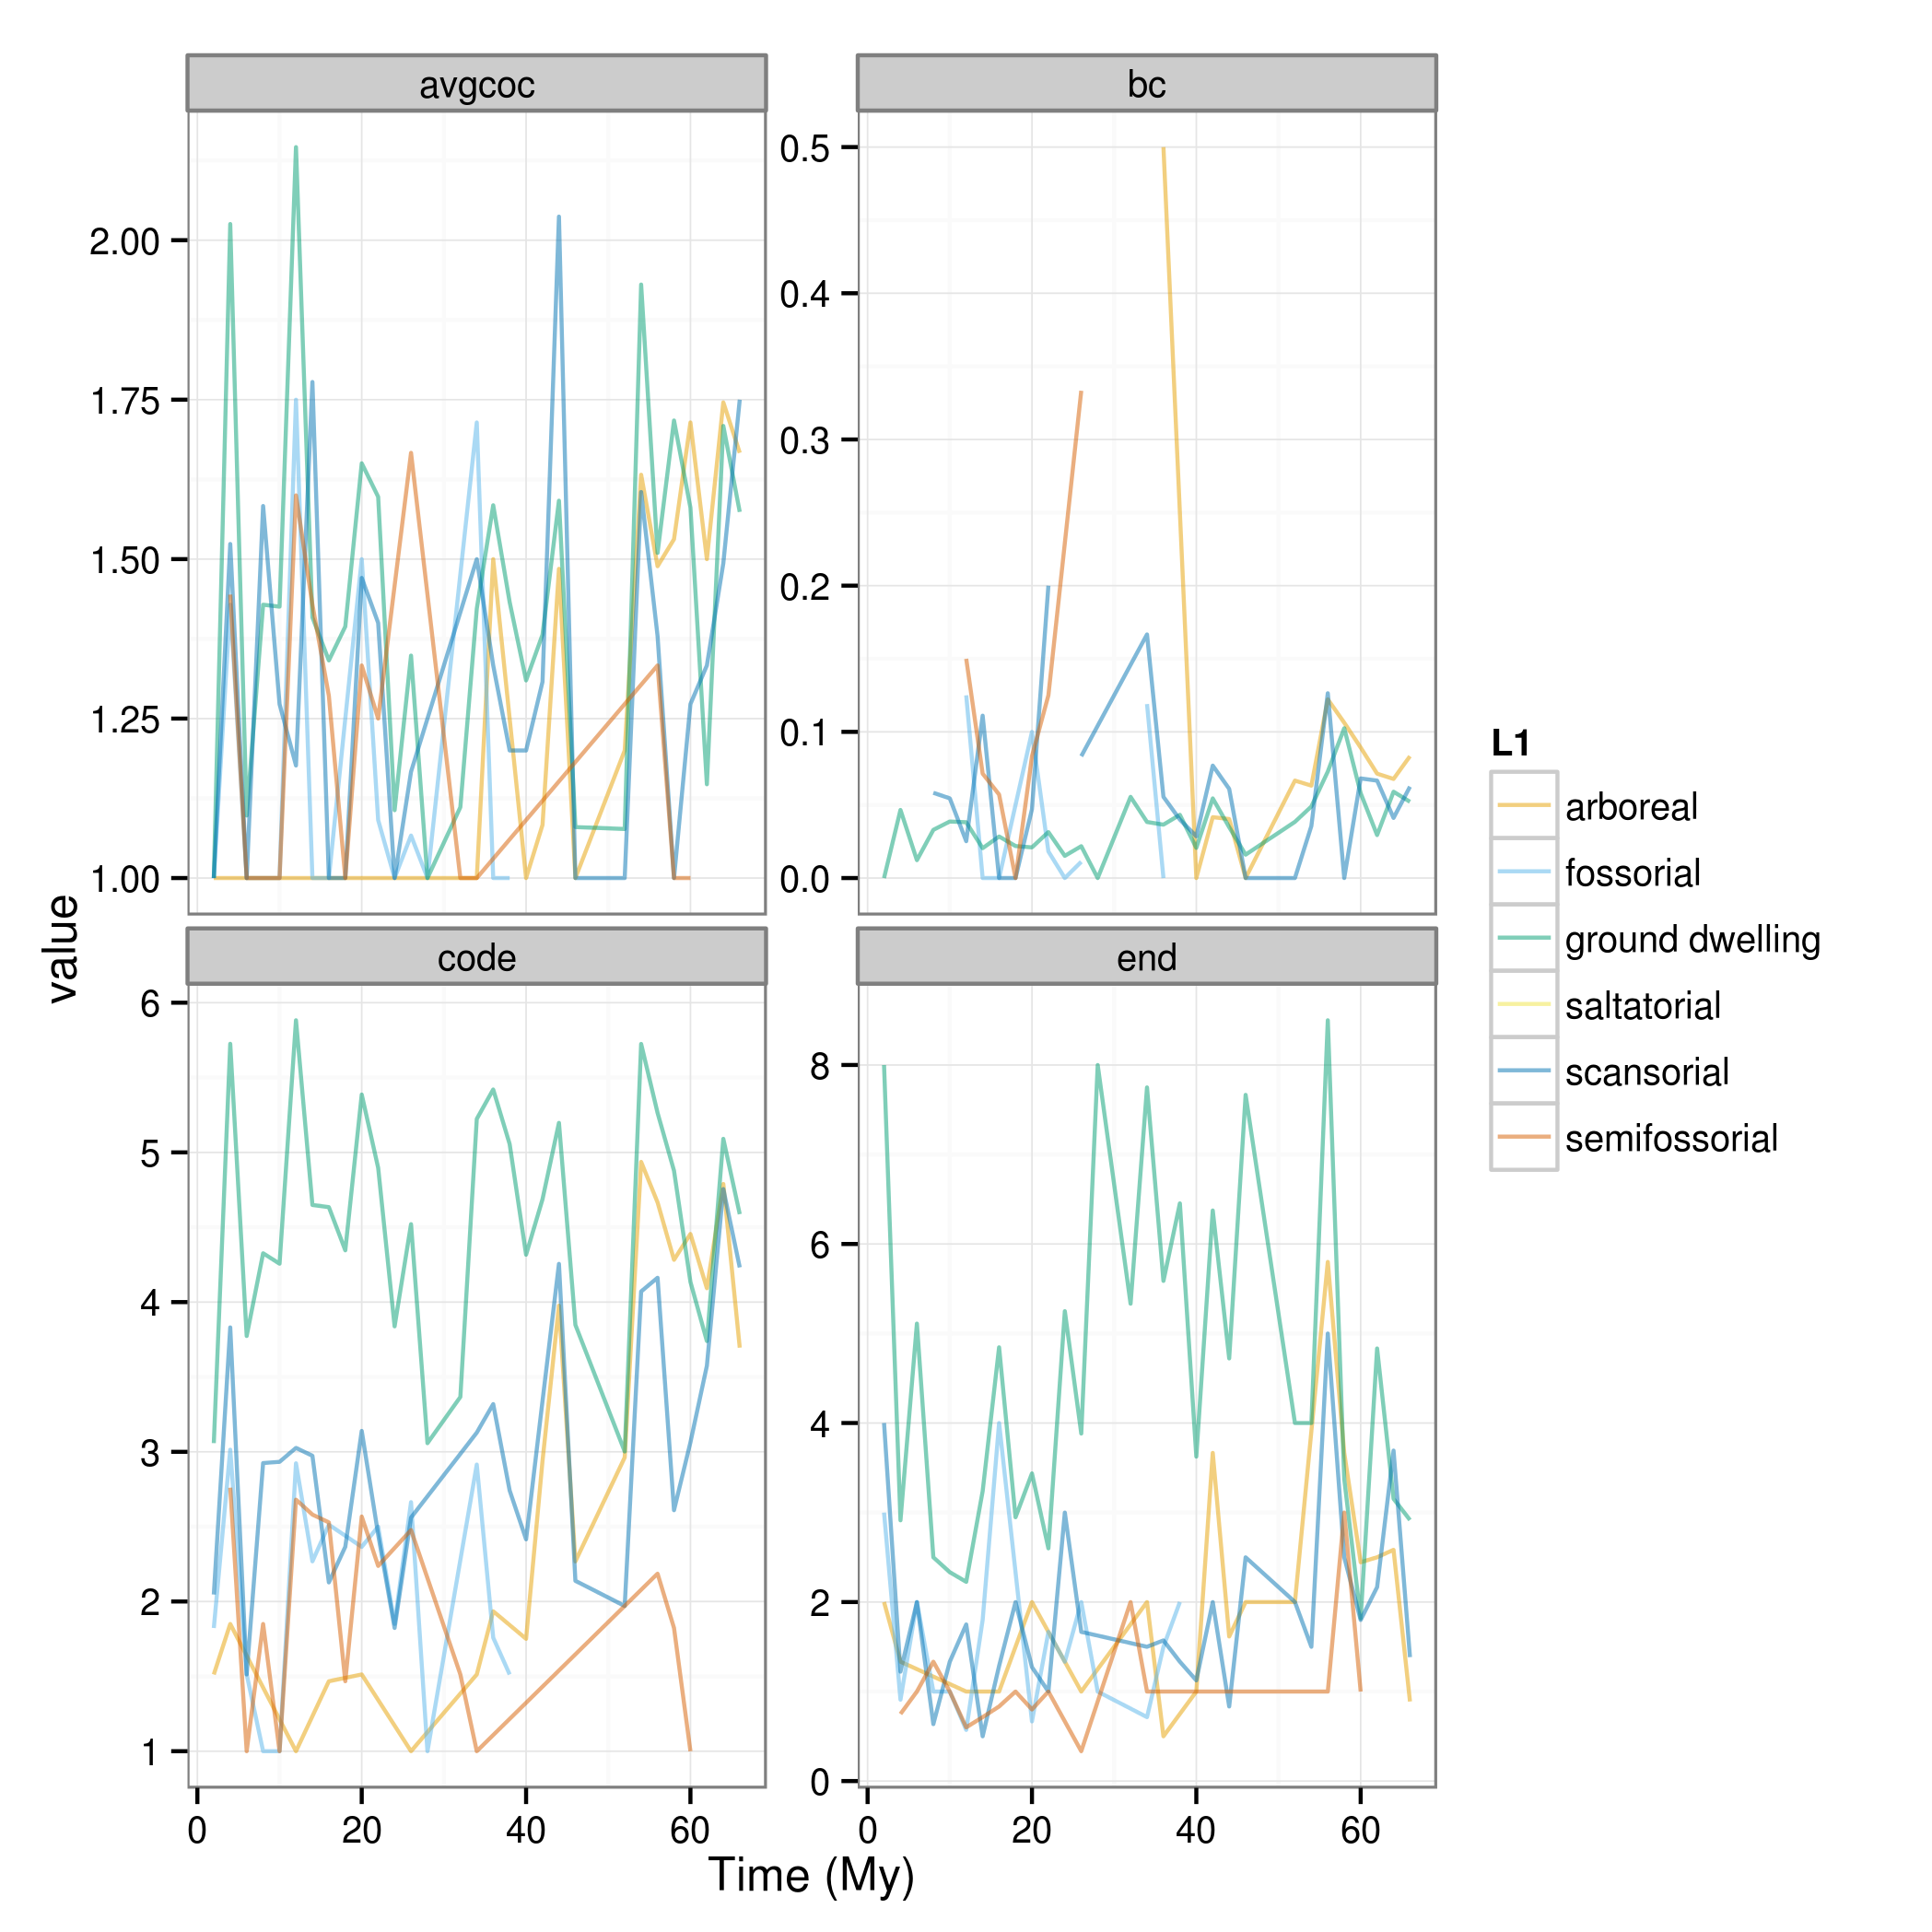
\includegraphics[width = 0.8\onecolwid]{figure/loco_bin}
              \label{fig:net_loco}
            \end{subfigure}
          \end{center}
          \caption{Biogeographic network summary statistics from the 2 My bins.}
          \label{fig:net_sum}
        \end{figure}
      \end{alertblock}

      \begin{columns}[t,totalwidth = \twocolwid]
        \begin{column}{\onecolwid}
          \begin{block}{Relative diet}
            \begin{figure}[ht]
              \centering
              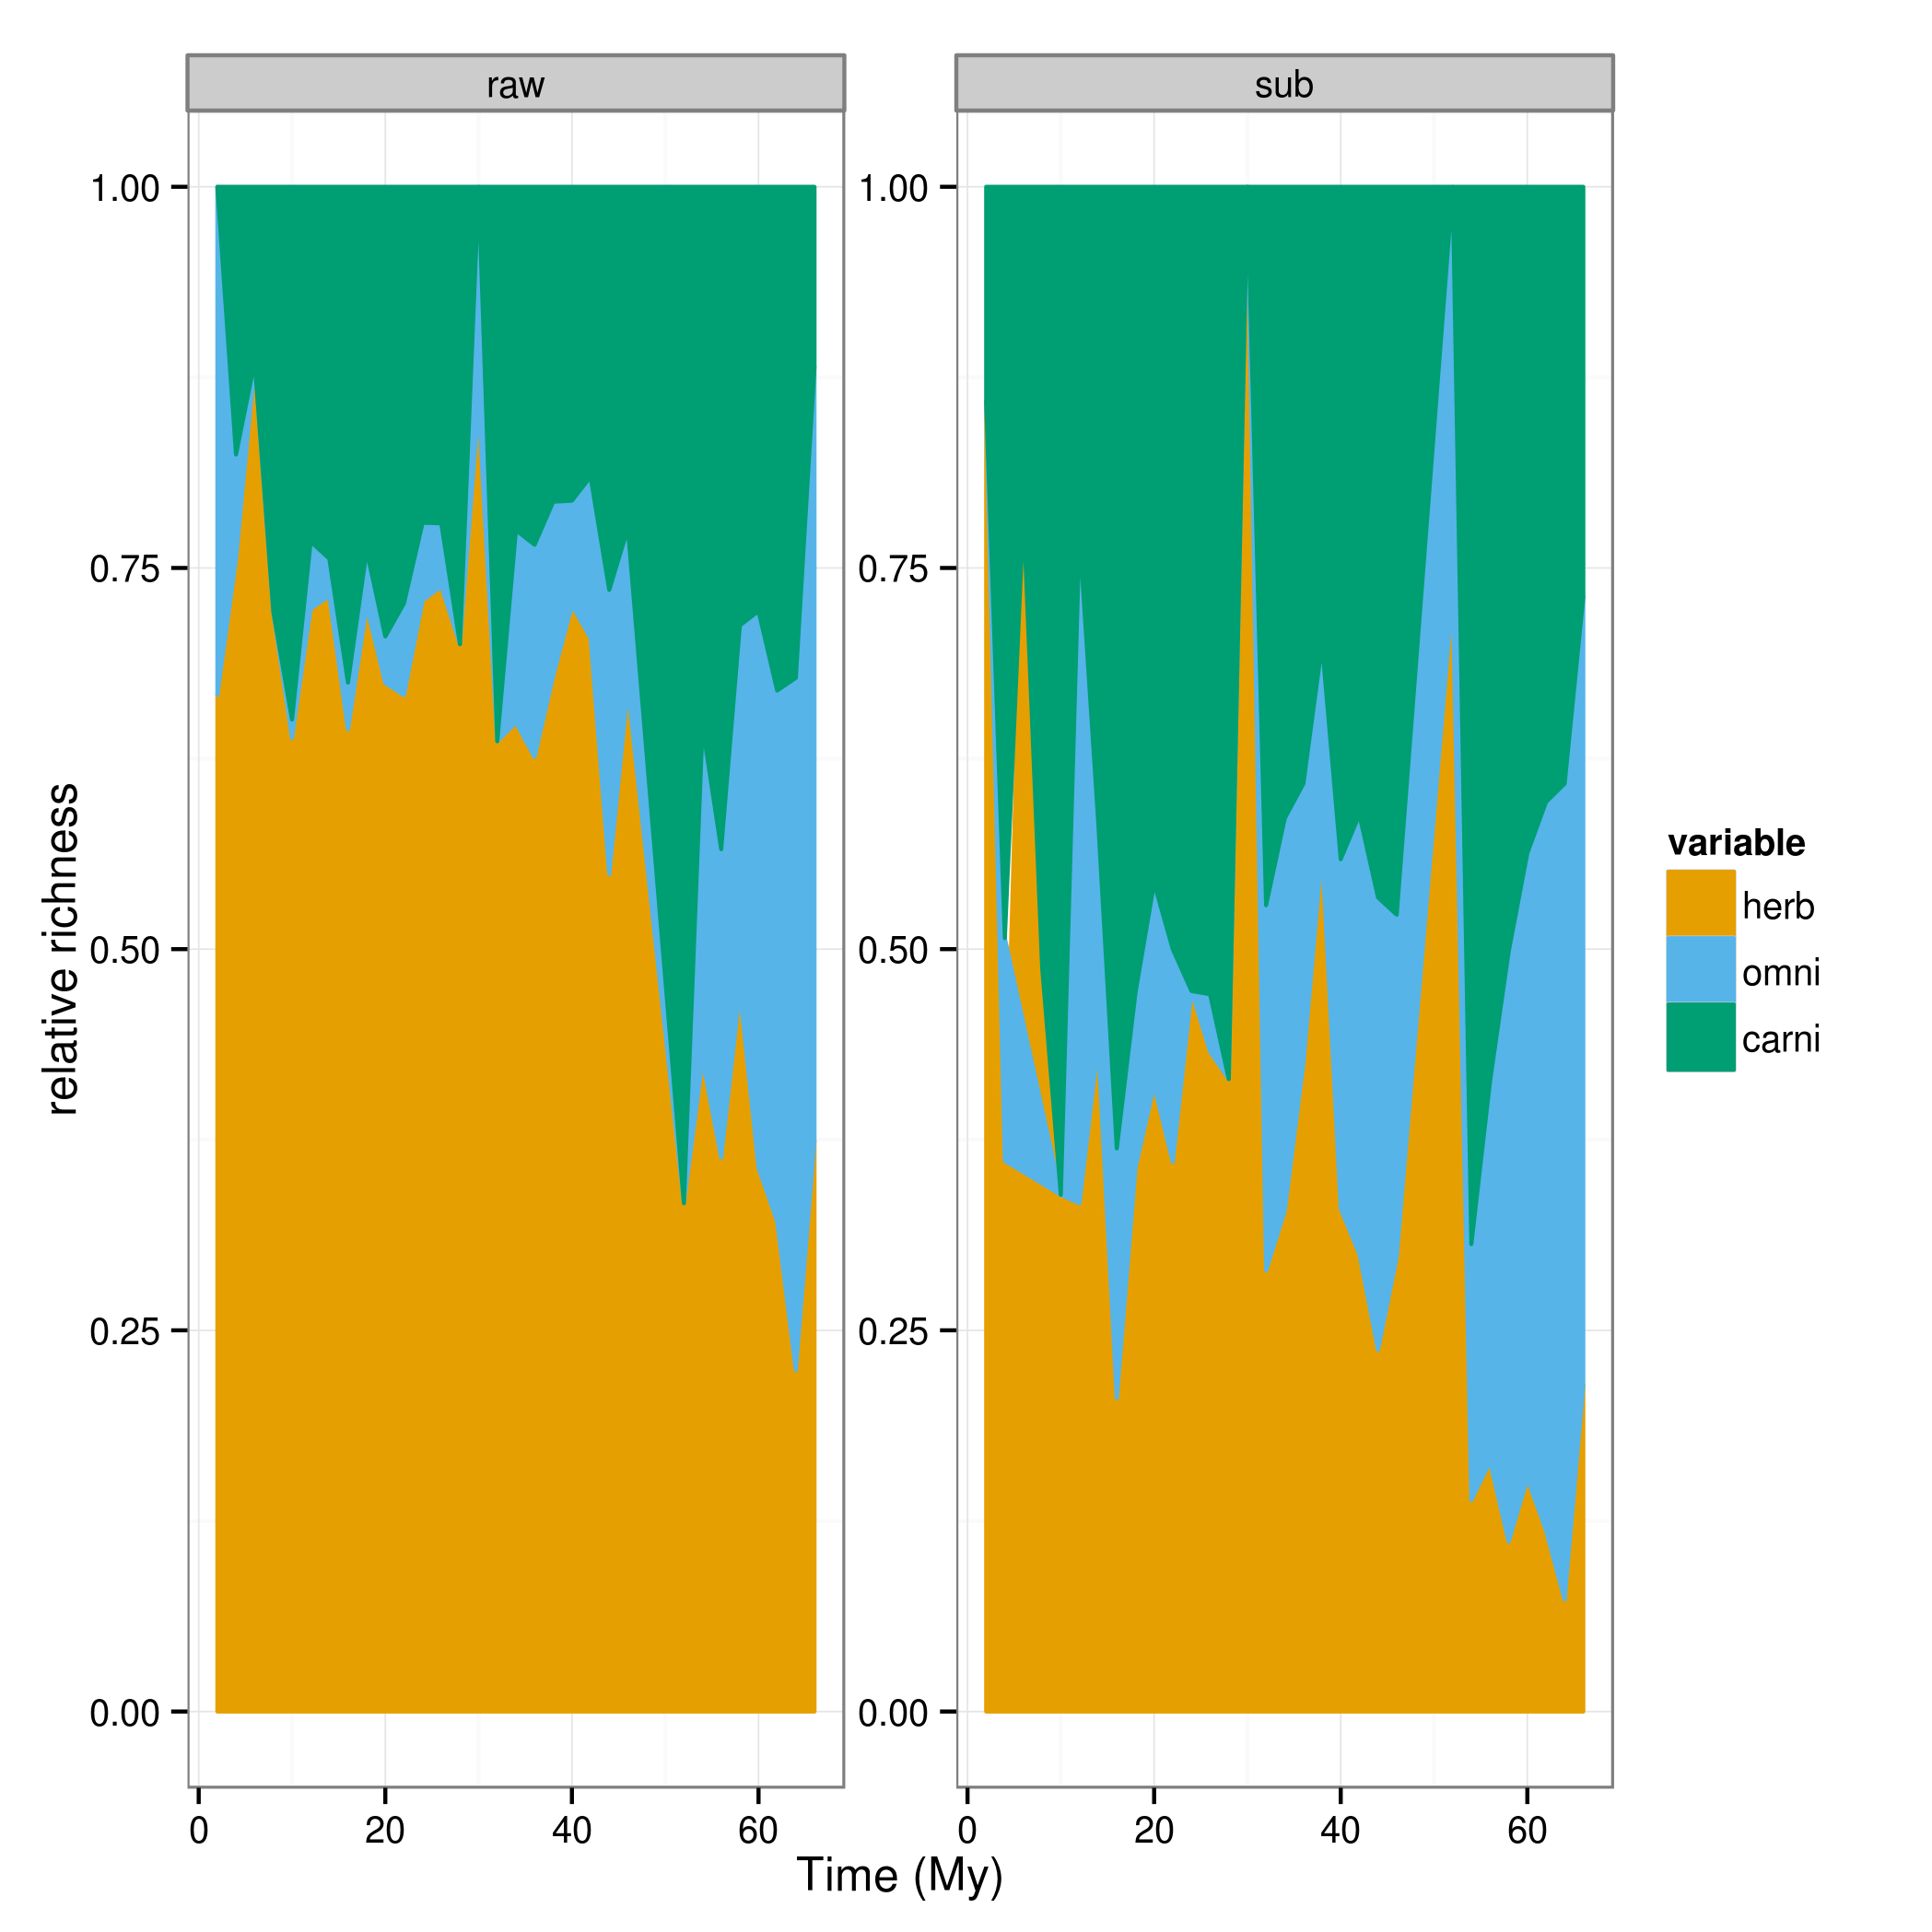
\includegraphics[height = 0.2\textheight]{figure/facet_mix}
              \caption{Relative abundance of mammalian dietary categories both raw and subsampled. Subsampled abundance was done using SQS.}
              \label{fig:rel_ab}
            \end{figure}
          \end{block}
        \end{column}

        \begin{column}{\onecolwid}
          \begin{block}{Diet ~ oxygen}
            \begin{figure}[ht]
              \centering
              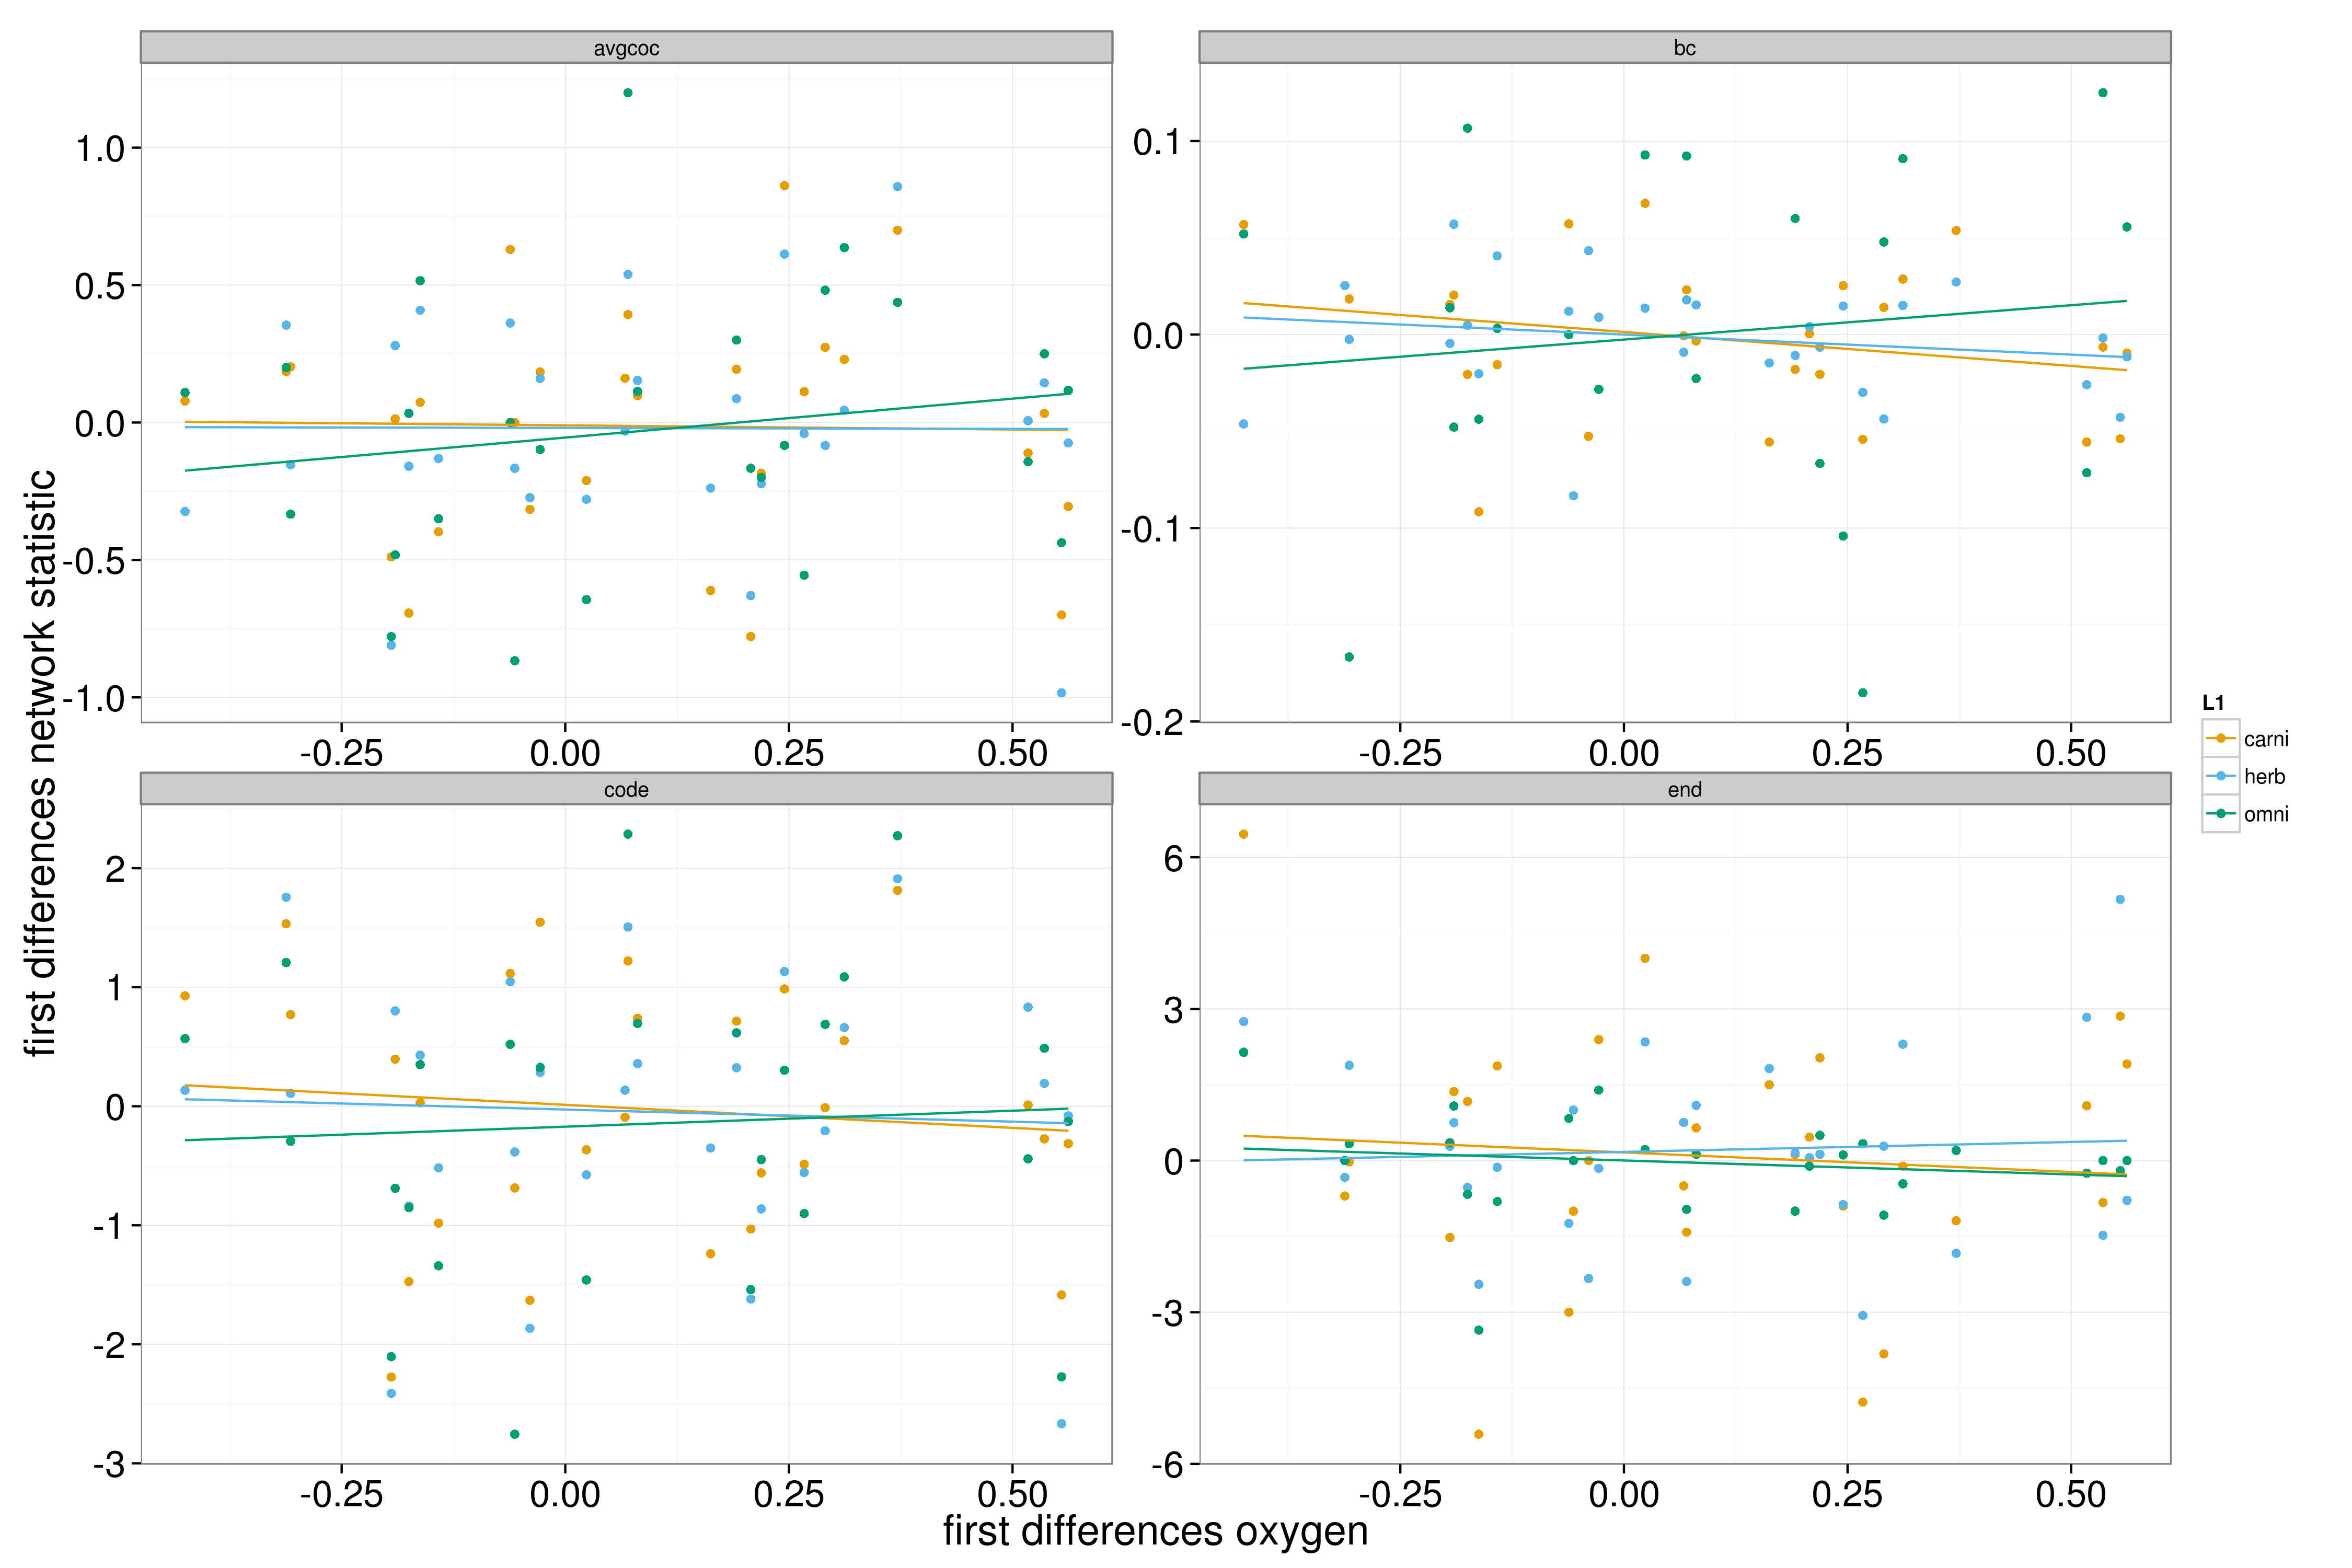
\includegraphics[height = 0.2\textheight]{figure/dt_oxy}
              \caption{Biplots of the first differences of the biogeographic network summary statistic time series versus the first differences of the binned \(\delta O^{18}\) isotope curve from \citep{Zachos2008}.}
              \label{fig:cor}
            \end{figure}
          \end{block}
        \end{column}
      \end{columns}


    \end{column}

    \begin{columns}[t,totalwidth = \onecolwid]
      \begin{column}{\onecolwid}
        \begin{block}{Discussion}
          \begin{itemize}
            \item generally stationary time series of biogeographic structure over Cenozoic (Fig. \ref{fig:net_gen})
            \begin{itemize}
              \item herbivore pattern is most similar to overall pattern, similar to \citet{Jernvall2002} and \citet{Jernvall2004}
              \item increase in relative proportion of herbivores (Fig. \ref{fig:rel_ab})
            \end{itemize}
            \item no correlation between oxygen and dietary (Fig. \ref{fig:cor}) or locomotor category (not shown)
              \begin{itemize}
                \item climate not a correlate/driver of NA-wide community structure over all Cenozoic
                \item life history traits plays stronger roll
              \end{itemize}
            \item preliminary correlation between dietary and locomotor categories (not shown)
          \end{itemize}
        \end{block}

        \begin{block}{Future directions}
          \begin{itemize}
            \item restrict to major orders \citep{Jernvall2004}
            \item reorganize locomotor categories (i.e. fewer)
            \begin{itemize}
              \item arboreal versus ground dwelling
            \end{itemize}
            \item account for difference in (relative) abundance (Fig. \ref{fig:rel_ab})
            \begin{itemize}
              \item maintenance of trophic structure \citep{Jernvall2004}?
              \item common taxa driving structure (ground-dwelling herbivores) \citep{Jernvall2002}?
            \end{itemize}
            \item is ecotype effect stronger than taxonomic effect?
          \end{itemize}
        \end{block}


        \begin{scriptsize}
          \begin{block}{Acknowledgements}
            I would like to thank John Alroy for helpful advice and kindly having compiled the (vast) majority of the occurence information used in this study. I would also like to thank my advisors Ken Angielczyk and Michael Foote for useful advice which greatly improved this study. 
            \begin{center}
              
\includegraphics[height = 0.1\textheight]{figure/chicago}
            \end{center}
          \end{block}
        \end{scriptsize}

        % bibliography
        \begin{scriptsize}
          \begin{block}{Bibliography}
            \bibliographystyle{abbrvnat}
            \bibliography{cosmo_prov,packages}
          \end{block}
        \end{scriptsize}

      \end{column}
    \end{columns}

  \end{columns}
\end{frame}
\end{document}
